%\clearpage

\section {Super-K samples used in the analysis}
\label{sec:samples}

This analysis is comprised of five samples based on the fiTQun selection algorithm, which has improved reconstruction capabilities and can therefore reduce the background components of the selected samples. The five samples are:
\begin{itemize}
	\item neutrino mode single $\mu$-like ring sample
	\item antineutrino mode single $\mu$-like ring sample
	\item neutrino mode single $e$-like ring sample
	\item antineutrino mode single $e$-like ring sample
	\item neutrino mode single $e$-like ring sample with one decay electron (referred to as \nueCConepi{})
\end{itemize}
The Super-K MC templates contain events from the $\nu_{\mu}$, $\bar{\nu}_{\mu}$, $\nu_{e}$, $\bar{\nu}_{e}$, oscillated $\nu_{e}$ and oscillated $\bar{\nu}_{e}$ samples passing the Super-K selection cuts. Details of the selection cuts can be found in \cite{Superk_run8}.

\subsection {Predicted event rates}
\label{sec:spectrum_prediction}
Predicted event rates for this analysis are determined for the case of two different sets of oscillation parameters based on previous best fit results from T2K and NOvA. These parameter sets are referred to as Asimov A and B, with their definitions and associated event rates given in the following sections.

\subsubsection{Definition of Asimov A and B}
\label{sec:asimov_definition}
%\Cref{tab:asimov_definition1} shows the definitions used for the Asimov data sets. Asimov A represents parameter values close to the T2K best fit for Run 1-7, whilst Asimov B modifies these parameters such that CP is conserved and uses NOvA's non-maximal mixing best fit value for \ssqthtwothree \cite{Adamson:2017nova}.
\Cref{tab:asimov_definition1} shows the definitions used for the Asimov data sets. Asimov A represents parameter values close to the T2K best fit for Run 1-7, whilst Asimov B modifies these parameters such that CP is conserved and changes the \ssqthtwothree octant.
\begin{table}[H]
\centering
\begin{tabular}{| c | c | c |}
\hline
Parameter(s) &	Asimov A & Asimov B	\\
\hline
$\sin^{2}\theta_{23}$	&	0.528	&  0.450	\\%0.624	\\
$\sin^{2} \theta_{13}$ reactors	&	0.0219	&	0.0219	\\
$\sin^{2} \theta_{12}$	&	0.304	&	0.304	\\
$|\Delta m^{2}_{32}|$ (NH) / $|\Delta m^{2}_{31}|$ (IH)	&	$2.509 \times 10^{-3}~\mbox{eV}^2/\mbox{c}^4$	&	$2.509 \times 10^{-3}~\mbox{eV}^2/\mbox{c}^4$	\\
$\Delta m^{2}_{21}$	&	$7.53 \times 10^{-5}~\mbox{eV}^2/\mbox{c}^4$	&	$7.53 \times 10^{-5}~\mbox{eV}^2/\mbox{c}^4$	\\
$\delta_{CP}$	&	-1.601	&	0	\\
Mass Hierarchy	&	Normal	&	Normal	\\  
\hline
\end{tabular}
\caption{
Values of oscillation parameters used to compute the event rates, systematic effects and sensitivity studies. Each set of oscillation parameters correspond to a different Asimov data set, which is the MC expected distribution in a certain oscillation hypothesis.
In the Asimov data set A the nominal values of $\sin^2 2 \theta_{13}$, $\sin^2 2 \theta_{12}$ and $\Delta m^2_{21}$  are from \cite{pdg_2014}, while all the other oscillation parameter values corresponds to the most probable values obtained by the Bayesian analysis on the T2K run 1-4 neutrino mode data \cite{T2KLongPaper}. The mass hierarchy is not marginalised but fixed to either NH or IH.
}
\label{tab:asimov_definition1}
\end{table}

\subsubsection{Event rates}
\label{sec:event_rates}
\Cref{tab:events_asimov_a_dcp_var_1re} shows the expected event rates in Super-K for the Asimov A data set, but with \deltacp varied at $-\pi/2$, 0, $\pi/2$ and $\pi$.
\begin{table}[H]
\center
\begin{tabular} { | l ||r | r | r | r | }
	\hline
	&	$\delta_{CP}=-\pi/2$	&	$\delta_{CP}=0$	&	$\delta_{CP}=\pi/2$	&	$\delta_{CP}=\pi$	\\ \hline\hline
	FHC $e$-like sample				& 73.47354  & 61.43388  & 49.90582  & 61.94533  \\ \hline
	FHC $\mu$-like sample			& 268.40351 & 268.05327 & 268.37281 & 268.81441 \\ \hline
	FHC \nueCConepi{}-like sample	& 6.92243   & 6.00922   & 4.86656   & 5.77983   \\ \hline
	RHC $e$-like sample				& 7.91206   & 9.02311   & 10.02989  & 8.91886   \\ \hline
	RHC $\mu$-like sample			& 64.27306  & 64.12292  & 64.27392  & 64.43654  \\ \hline	
\end{tabular}
\caption{
%{\Huge{TO UPDATE}}
Predicted total number of events in each sample obtained after applying the BANFF weight for a total exposure of \TotalPotNu{} POT. The Asimov data set A in \ref{tab:asimov_definition1} is used, but with varying \deltacp.
}
\label{tab:events_asimov_a_dcp_var_1re}
\end{table}


\Crefrange{tab:events_1rmu_Asimov_A}{tab:events_cconepi_Asimov_A} present the expected event rates in Super-K corresponding to the Asimov A data set. Event rates in other oscillation scenarios can be found in \cref{app:event_rates}. In each case the normal hierarchy is assumed and all rates are generated for an integrated exposure corresponding to \RunPeriod.

\begin{table}[H]
\center
\begin{tabular} { | l ||r | r | r | r | r | r | | r | }
\hline
              & $\nu_\mu$            & $\nu_e$              & $\bar{\nu}_{\mu}$    & $\bar{\nu}_{e}$      & Osc. $\nu_e$         & Osc. $\bar{\nu}_{e}$ & Total                \\ \hline\hline
 CCQE         & 175.62883            & 0.00413              & 11.03473             & 0.00019              & 0.02245              & 0.00015              & 186.69049            \\ \hline
 CC1pi        & 27.69898             & 0.00199              & 2.61604              & 0.00009              & 0.02406              & 0.00007              & 30.34123             \\ \hline
 CCcoherent   & 0.28837              & 0.00000              & 0.09218              & 0.00000              & 0.00000              & 0.00000              & 0.38055              \\ \hline
 2p2h         & 35.57284             & 0.00151              & 1.41213              & 0.00008              & 0.02551              & 0.00004              & 37.01211             \\ \hline
 CCother      & 5.46647              & 0.00086              & 0.40615              & 0.00008              & 0.00011              & 0.00001              & 5.87368              \\ \hline
 NC1pi0       & 0.61495              & 0.01841              & 0.02120              & 0.00143              & N/A                  & N/A                  & 0.65599              \\ \hline
 NC1piPM      & 4.90783              & 0.09799              & 0.17531              & 0.00975              & N/A                  & N/A                  & 5.19089              \\ \hline
 NCcoherent   & 0.00000              & 0.00000              & 0.00043              & 0.00003              & N/A                  & N/A                  & 0.00047              \\ \hline
 NCother      & 2.05619              & 0.07378              & 0.13055              & 0.00912              & N/A                  & N/A                  & 2.26963              \\ \hline
\hline
 Total        & 252.23446            & 0.19867              & 15.88872             & 0.02078              & 0.07214              & 0.00027              & 268.41504            \\ \hline

\end{tabular}

\caption{
%{\Huge{TO UPDATE}}
Predicted number of events in the neutrino mode $\mu$-like sample obtained after applying the BANFF weight for a total exposure of \TotalPotNu{} POT. The Asimov data set A in \ref{tab:asimov_definition1} is used.
}
\label{tab:events_1rmu_Asimov_A}
\end{table}




\begin{table}[H]
\center
\begin{tabular} { | l ||r | r | r | r | r | r | | r | }
\hline
              & $\nu_\mu$            & $\nu_e$              & $\bar{\nu}_{\mu}$    & $\bar{\nu}_{e}$      & Osc. $\nu_e$         & Osc. $\bar{\nu}_{e}$ & Total                \\ \hline\hline
 CCQE         & 15.29349             & 0.00085              & 29.88622             & 0.00093              & 0.00094              & 0.00137              & 45.18379             \\ \hline
 CC1pi        & 3.95485              & 0.00033              & 4.53265              & 0.00025              & 0.00060              & 0.00061              & 8.48929              \\ \hline
 CCcoherent   & 0.04705              & 0.00000              & 0.17567              & 0.00005              & 0.00000              & 0.00006              & 0.22283              \\ \hline
 2p2h         & 4.47453              & 0.00026              & 2.84291              & 0.00027              & 0.00044              & 0.00021              & 7.31861              \\ \hline
 CCother      & 0.94199              & 0.00012              & 0.60584              & 0.00000              & 0.00000              & 0.00000              & 1.54795              \\ \hline
 NC1pi0       & 0.06000              & 0.00222              & 0.06147              & 0.00169              & N/A                  & N/A                  & 0.12538              \\ \hline
 NC1piPM      & 0.35950              & 0.01527              & 0.46009              & 0.01235              & N/A                  & N/A                  & 0.84721              \\ \hline
 NCcoherent   & 0.00000              & 0.00000              & 0.00201              & 0.00000              & N/A                  & N/A                  & 0.00201              \\ \hline
 NCother      & 0.31580              & 0.01640              & 0.20064              & 0.00789              & N/A                  & N/A                  & 0.54073              \\ \hline
\hline
 Total        & 25.44720             & 0.03544              & 38.76749             & 0.02342              & 0.00198              & 0.00226              & 64.27780             \\ \hline

\end{tabular}

\caption{
%{\Huge{TO UPDATE}}
Predicted number of events in the antineutrino mode $\mu$-like sample obtained after applying the BANFF weight for a total exposure of \TotalPotNuBar{} POT. The Asimov data set A in \ref{tab:asimov_definition1} is used.
}
\label{tab:events_rhc1rmu_Asimov_A}
\end{table}




\begin{table}[H]
\center
\begin{tabular} { | l ||r | r | r | r | r | r | | r | }
\hline
              & $\nu_\mu$            & $\nu_e$              & $\bar{\nu}_{\mu}$    & $\bar{\nu}_{e}$      & Osc. $\nu_e$         & Osc. $\bar{\nu}_{e}$ & Total                \\ \hline\hline
 CCQE         & 0.16115              & 6.30178              & 0.00634              & 0.25566              & 46.25561             & 0.27811              & 53.25866             \\ \hline
 CC1pi        & 0.04703              & 0.93168              & 0.00280              & 0.06750              & 4.49505              & 0.04745              & 5.59150              \\ \hline
 CCcoherent   & 0.00011              & 0.00830              & 0.00018              & 0.00397              & 0.03445              & 0.00327              & 0.05028              \\ \hline
 2p2h         & 0.03033              & 1.59694              & 0.00117              & 0.04275              & 8.68112              & 0.03893              & 10.39125             \\ \hline
 CCother      & 0.01329              & 0.12803              & 0.00034              & 0.00942              & 0.08850              & 0.00326              & 0.24284              \\ \hline
 NC1pi0       & 1.70203              & 0.03706              & 0.06012              & 0.00356              & N/A                  & N/A                  & 1.80278              \\ \hline
 NC1piPM      & 0.16854              & 0.00472              & 0.01020              & 0.00057              & N/A                  & N/A                  & 0.18404              \\ \hline
 NCcoherent   & 0.52817              & 0.00715              & 0.04794              & 0.00294              & N/A                  & N/A                  & 0.58619              \\ \hline
 NCother      & 0.31767              & 0.01695              & 0.02120              & 0.00128              & N/A                  & N/A                  & 0.35711              \\ \hline
 NC1gamma     & 0.94222              & 0.01687              & 0.04983              & 0.00233              & N/A                  & N/A                  & 1.01125              \\ \hline
\hline
 Total        & 3.91054              & 9.04948              & 0.20014              & 0.38998              & 59.55473             & 0.37103              & 73.47589             \\ \hline

\end{tabular}

\caption{
%{\Huge{TO UPDATE}}
Predicted number of events in the neutrino mode $e$-like sample obtained after applying the BANFF weight for a total exposure of \TotalPotNuRunOneEight{} POT. The Asimov data set A in \ref{tab:asimov_definition1} is used.
}
\label{tab:events_1re_Asimov_A}
\end{table}




\begin{table}[H]
\center
\begin{tabular} { | l ||r | r | r | r | r | r | | r | }
\hline
              & $\nu_\mu$            & $\nu_e$              & $\bar{\nu}_{\mu}$    & $\bar{\nu}_{e}$      & Osc. $\nu_e$         & Osc. $\bar{\nu}_{e}$ & Total                \\ \hline\hline
 CCQE         & 0.01288              & 0.50911              & 0.02388              & 0.84721              & 1.02586              & 2.85198              & 5.27090              \\ \hline
 CC1pi        & 0.00763              & 0.10111              & 0.00733              & 0.14431              & 0.14337              & 0.33485              & 0.73858              \\ \hline
 CCcoherent   & 0.00002              & 0.00099              & 0.00042              & 0.01066              & 0.00114              & 0.03130              & 0.04455              \\ \hline
 2p2h         & 0.00295              & 0.14379              & 0.00219              & 0.11301              & 0.23285              & 0.33042              & 0.82521              \\ \hline
 CCother      & 0.00390              & 0.02116              & 0.00120              & 0.01154              & 0.01042              & 0.00668              & 0.05491              \\ \hline
 NC1pi0       & 0.13849              & 0.00541              & 0.17659              & 0.00468              & N/A                  & N/A                  & 0.32516              \\ \hline
 NC1piPM      & 0.02475              & 0.00127              & 0.02001              & 0.00080              & N/A                  & N/A                  & 0.04683              \\ \hline
 NCcoherent   & 0.04776              & 0.00221              & 0.20260              & 0.00317              & N/A                  & N/A                  & 0.25574              \\ \hline
 NCother      & 0.05664              & 0.00221              & 0.02672              & 0.00097              & N/A                  & N/A                  & 0.08654              \\ \hline
 NC1gamma     & 0.07943              & 0.00439              & 0.17490              & 0.00383              & N/A                  & N/A                  & 0.26255              \\ \hline
\hline
 Total        & 0.37445              & 0.79164              & 0.63583              & 1.14019              & 1.41363              & 3.55523              & 7.91097              \\ \hline

\end{tabular}

\caption{
%{\Huge{TO UPDATE}}
Predicted number of events in the antineutrino mode $e$-like sample obtained after applying the BANFF weight for a total exposure of \TotalPotNu{} POT. The Asimov data set A in \ref{tab:asimov_definition1} is used.
}
\label{tab:events_rhc1re_Asimov_A}
\end{table}




\begin{table}[H]
\center
\begin{tabular} { | l ||r | r | r | r | r | r | | r | }
\hline
              & $\nu_\mu$            & $\nu_e$              & $\bar{\nu}_{\mu}$    & $\bar{\nu}_{e}$      & Osc. $\nu_e$         & Osc. $\bar{\nu}_{e}$ & Total                \\ \hline\hline
 CCQE         & 0.02857              & 0.02442              & 0.00117              & 0.00174              & 0.21123              & 0.00265              & 0.26979              \\ \hline
 CC1pi        & 0.07582              & 0.76065              & 0.00257              & 0.00383              & 4.85325              & 0.00227              & 5.69839              \\ \hline
 CCcoherent   & 0.00027              & 0.01765              & 0.00008              & 0.00007              & 0.11121              & 0.00011              & 0.12939              \\ \hline
 2p2h         & 0.01012              & 0.02195              & 0.00049              & 0.00095              & 0.16017              & 0.00105              & 0.19473              \\ \hline
 CCother      & 0.03770              & 0.11225              & 0.00116              & 0.00279              & 0.12085              & 0.00150              & 0.27625              \\ \hline
 NC1pi0       & 0.02049              & 0.00076              & 0.00083              & 0.00008              & N/A                  & N/A                  & 0.02216              \\ \hline
 NC1piPM      & 0.06474              & 0.00165              & 0.00382              & 0.00033              & N/A                  & N/A                  & 0.07053              \\ \hline
 NCother      & 0.20584              & 0.00830              & 0.01304              & 0.00088              & N/A                  & N/A                  & 0.22807              \\ \hline
 NC1gamma     & 0.02844              & 0.00000              & 0.00067              & 0.00007              & N/A                  & N/A                  & 0.02918              \\ \hline
\hline
 Total        & 0.47199              & 0.94764              & 0.02382              & 0.01075              & 5.45671              & 0.00758              & 6.91850              \\ \hline

\end{tabular}

\caption{
Predicted number of events in the neutrino mode \nueCConepi{}-like sample obtained after applying the BANFF weight
for a total exposure of \TotalPotNu{} POT. The Asimov data set A in \ref{tab:asimov_definition1} is used.
}
\label{tab:events_cconepi_Asimov_A}
\end{table}




\subsubsection{Predicted and observed spectra}
\label{sec:selection:predicted_spectra}

In this section, we present the expected spectra in Super-K for Asimov A and unoscillated scenarios, assuming normal hierarchy. All plots are generated for an integrated exposure corresponding to \RunPeriod.

Predicted single ring Super-K spectra are shown in \cref{fig:unosc_spectra_all,fig:asimova_spectra_all}. 
By comparing neutrino and antineutrino mode $e$-like plots it is clear that $\theta$ vs $E_{reco}$ distributions are differently populated by $\nu_{\mu} \rightarrow \nu_e$ and $\bar{\nu}_{\mu} \rightarrow \bar{\nu}_e$ events.

\begin{figure*}[htb]
	\center
	\begin{subfigure}[b]{0.49\textwidth}
		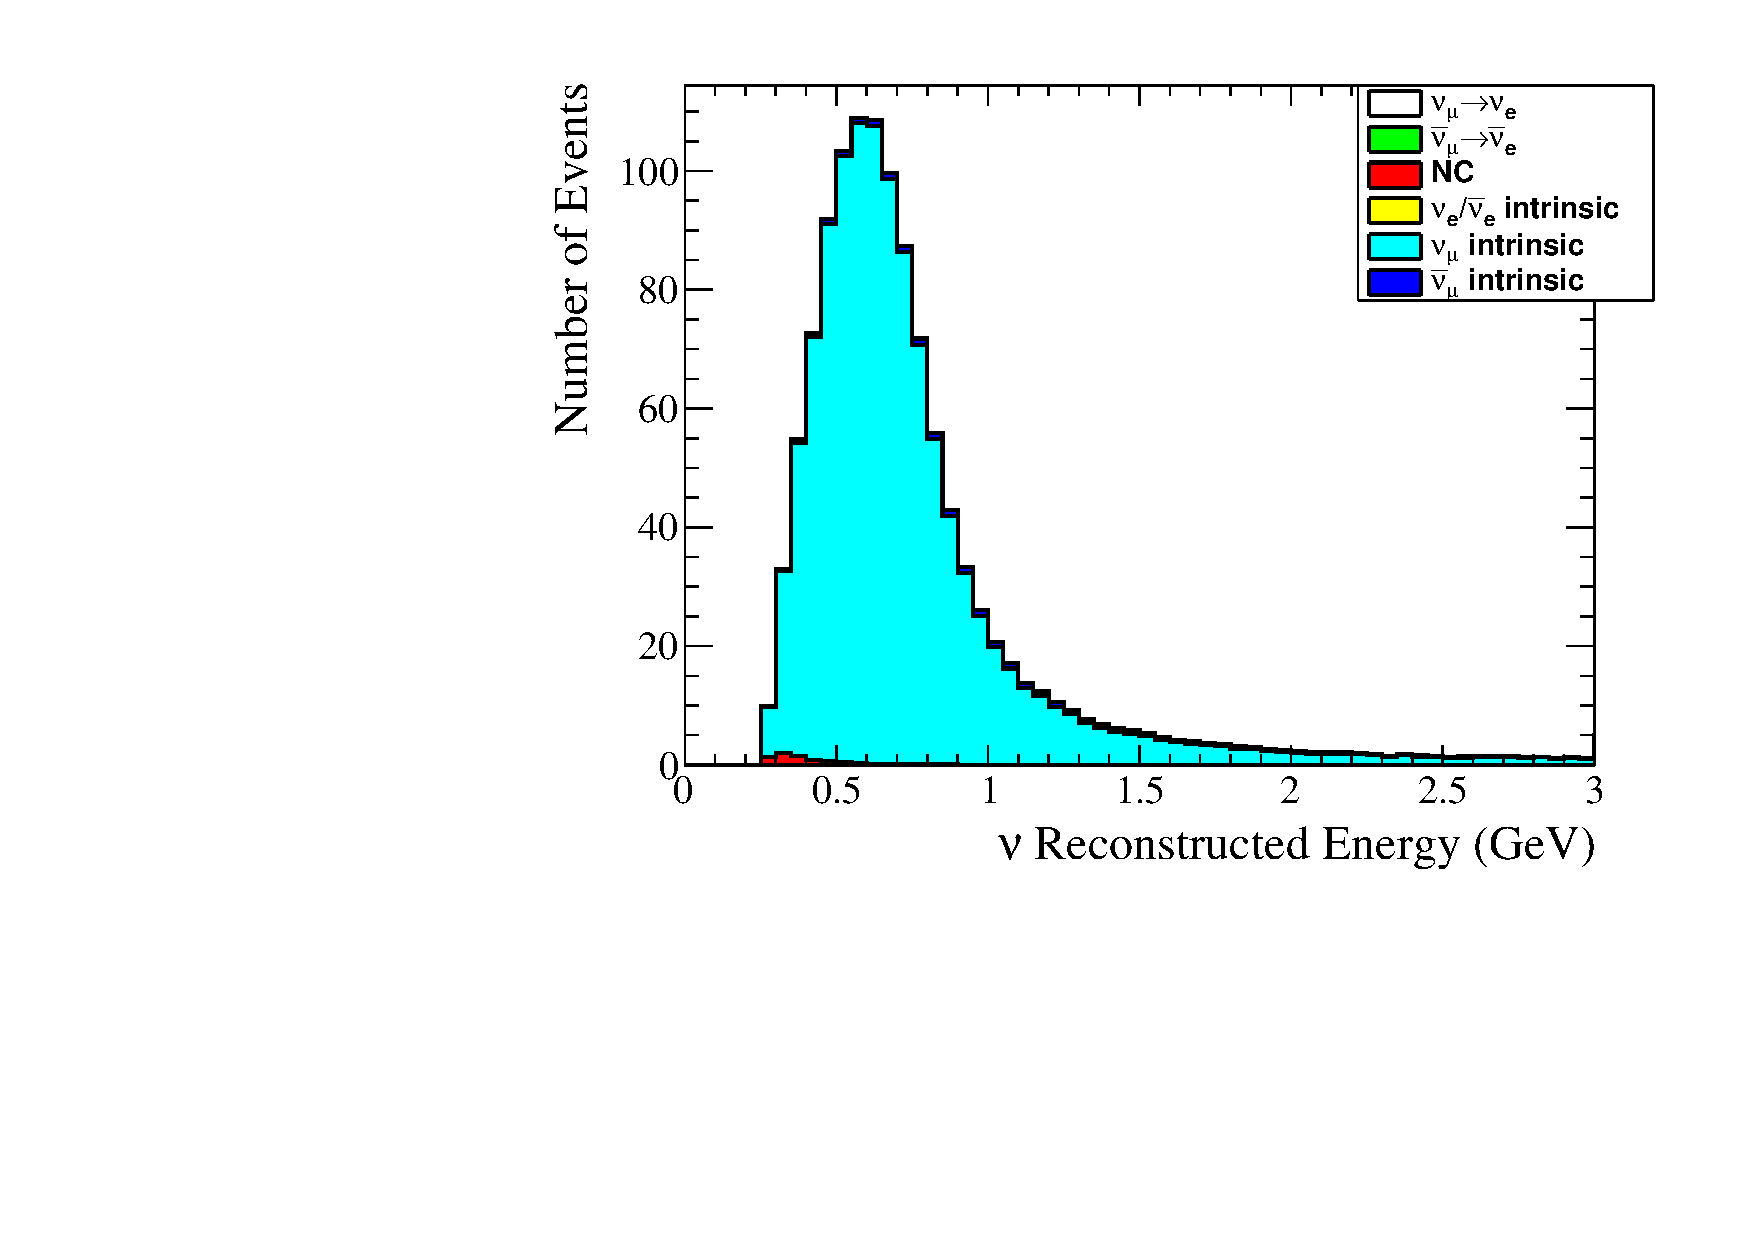
\includegraphics[width=0.9\textwidth]{spectra/spectrum_unosc_1Rmu}
		\caption{Muon-like, neutrino mode}
	\end{subfigure}
	\begin{subfigure}[b]{0.49\textwidth}
		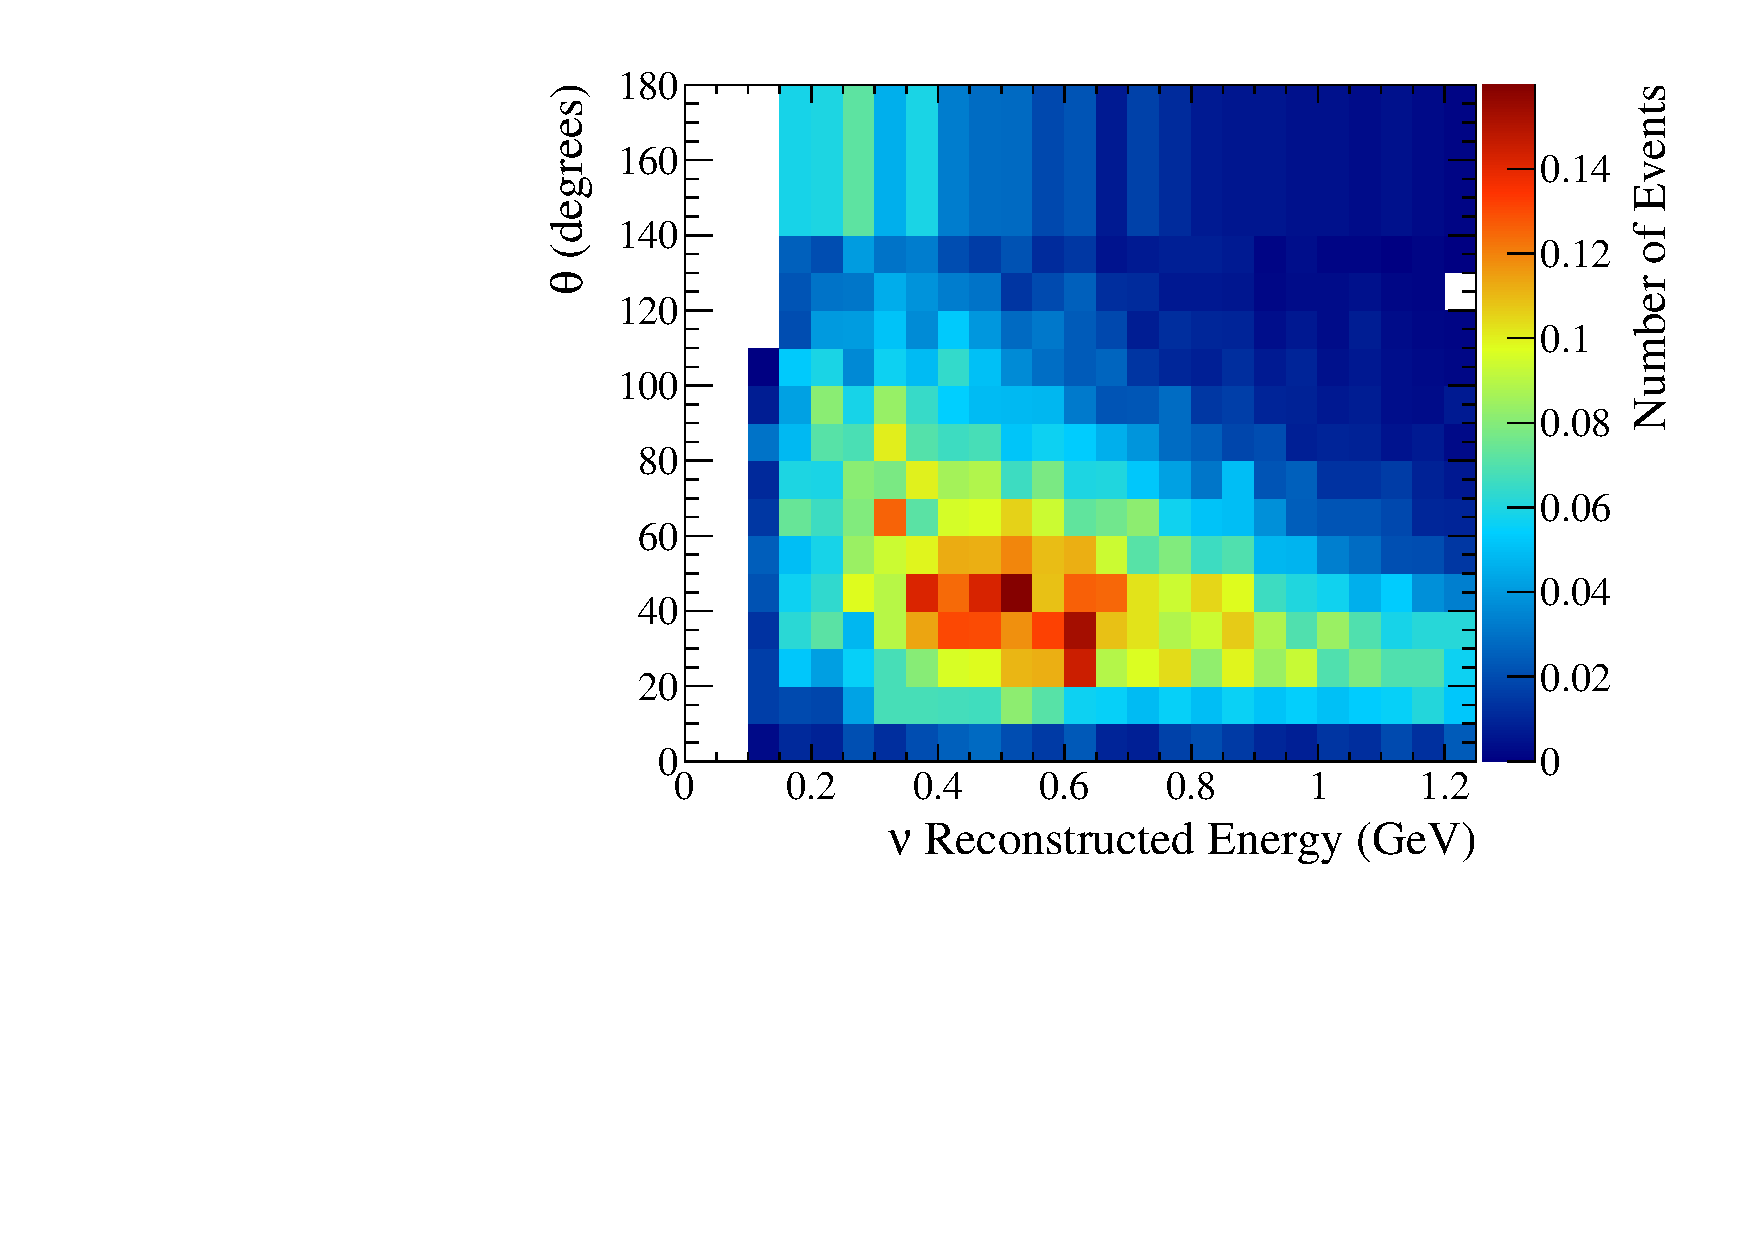
\includegraphics[width=0.9\textwidth]{spectra/spectrum_unosc_1Re}
		\caption{Electron-like, neutrino mode}
	\end{subfigure}
	\begin{subfigure}[b]{0.49\textwidth}
		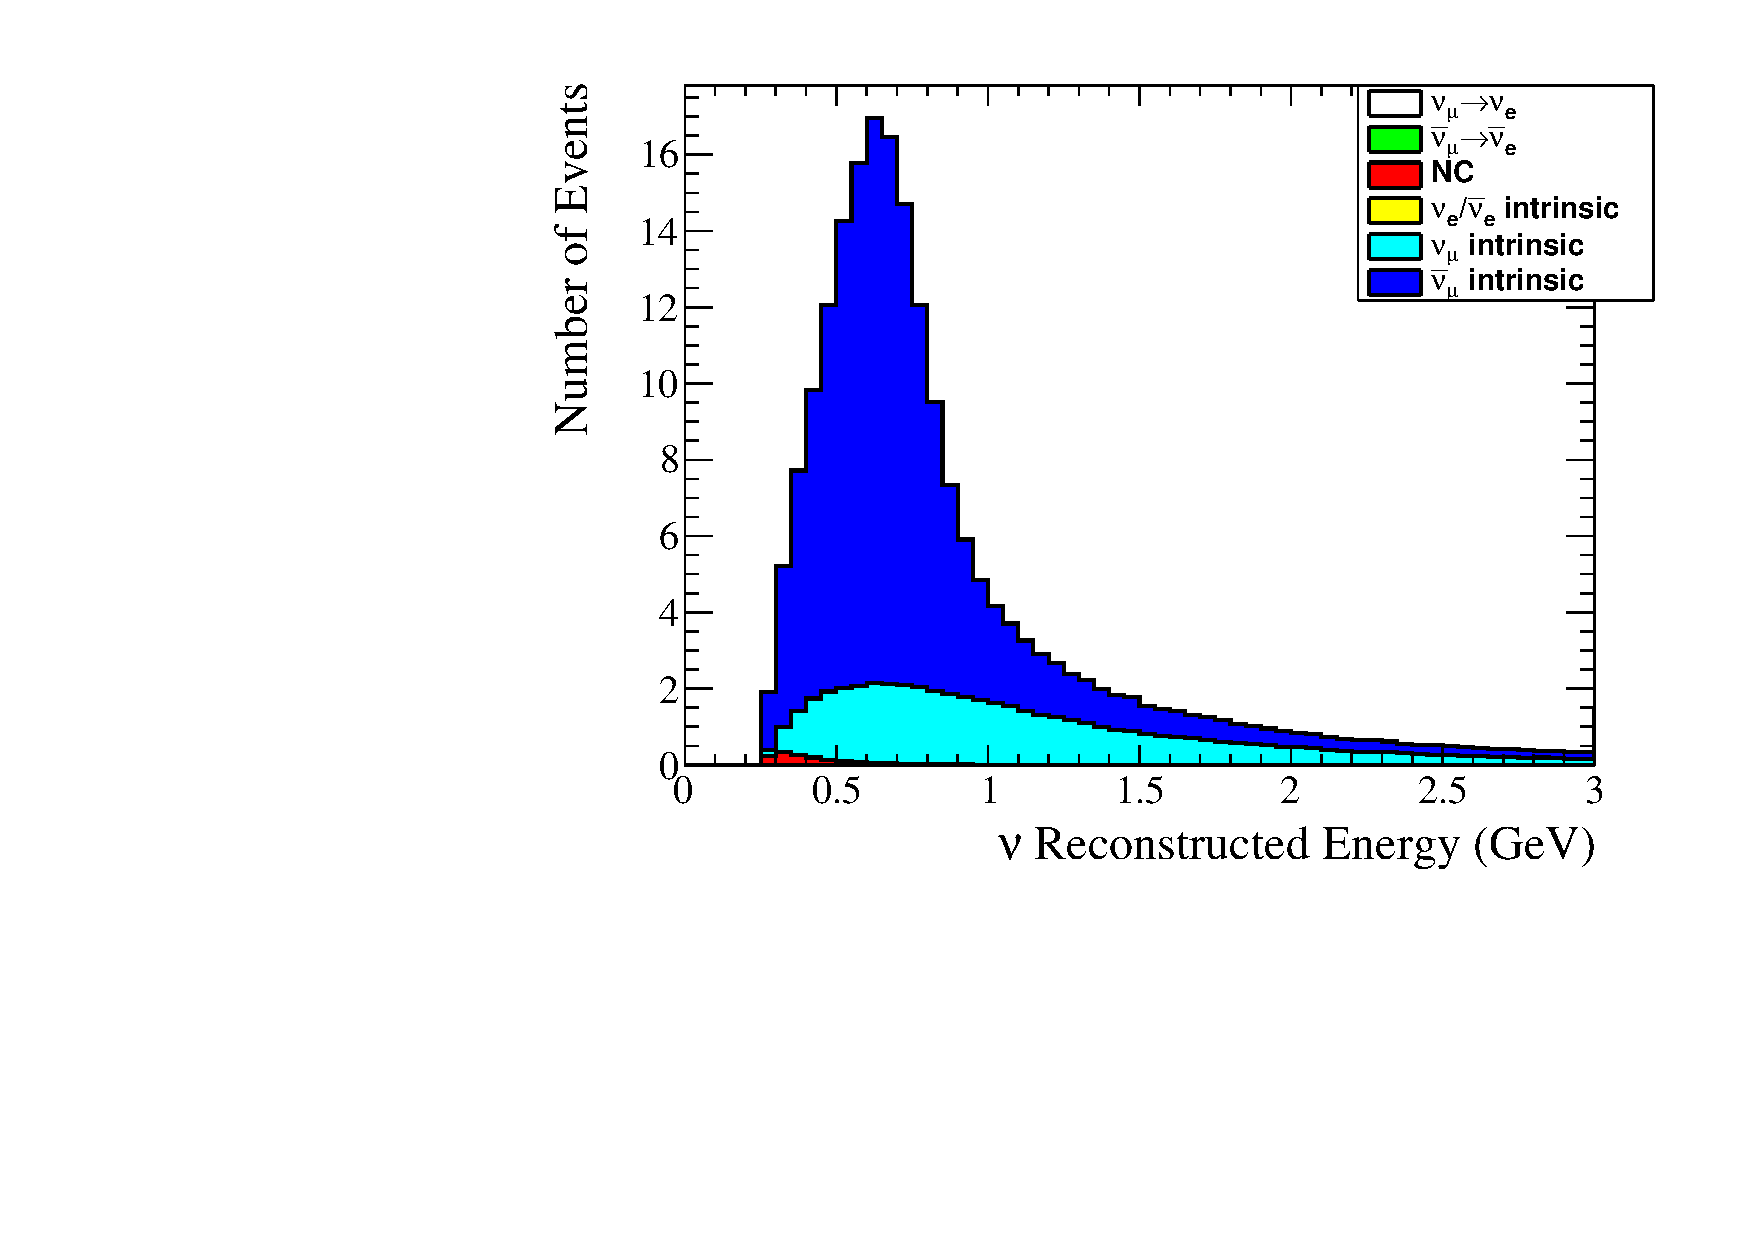
\includegraphics[width=0.9\textwidth]{spectra/spectrum_unosc_RHC1Rmu}
		\caption{Muon-like, antineutrino mode}
	\end{subfigure}
	\begin{subfigure}[b]{0.49\textwidth}
		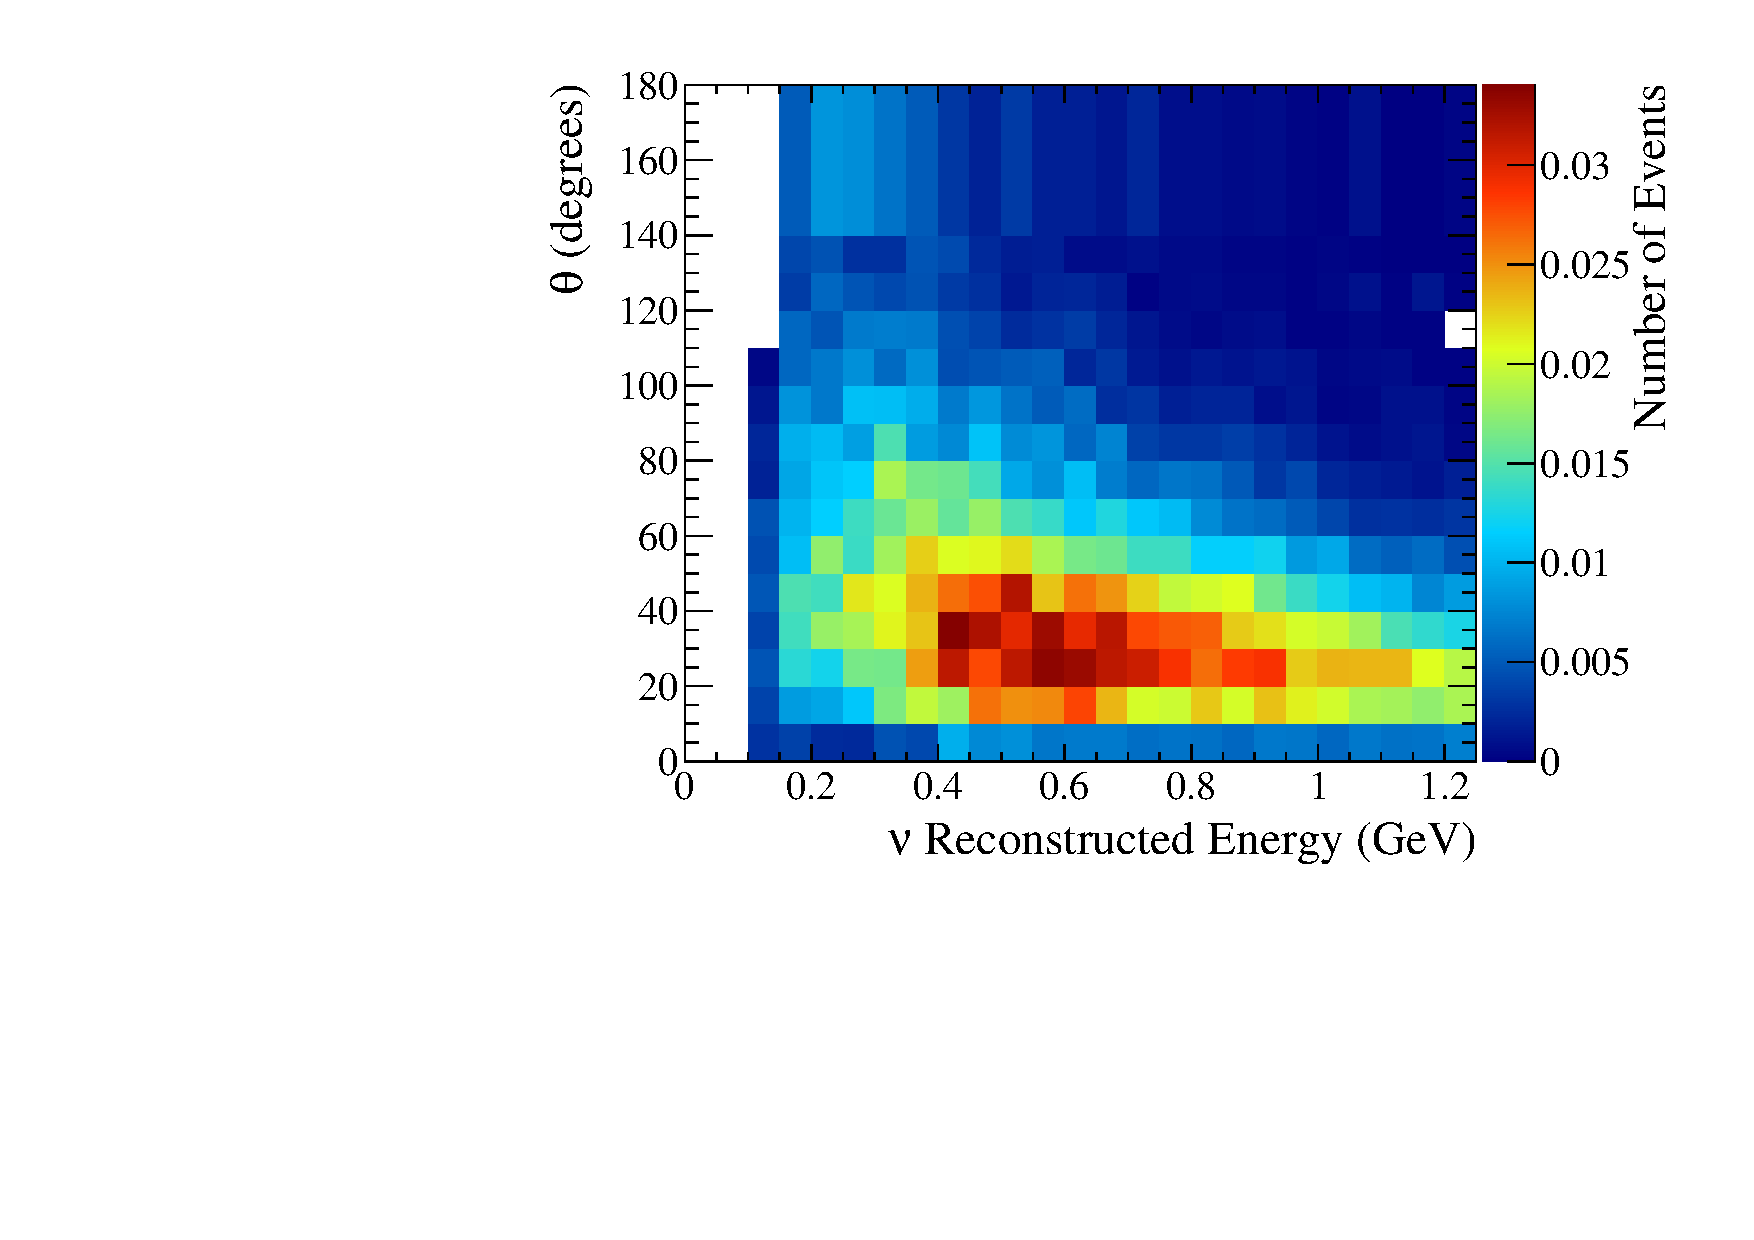
\includegraphics[width=0.9\textwidth]{spectra/spectrum_unosc_RHC1Re}
		\caption{Electron-like antineutrino mode}
	\end{subfigure}
	\begin{subfigure}[b]{0.49\textwidth}
		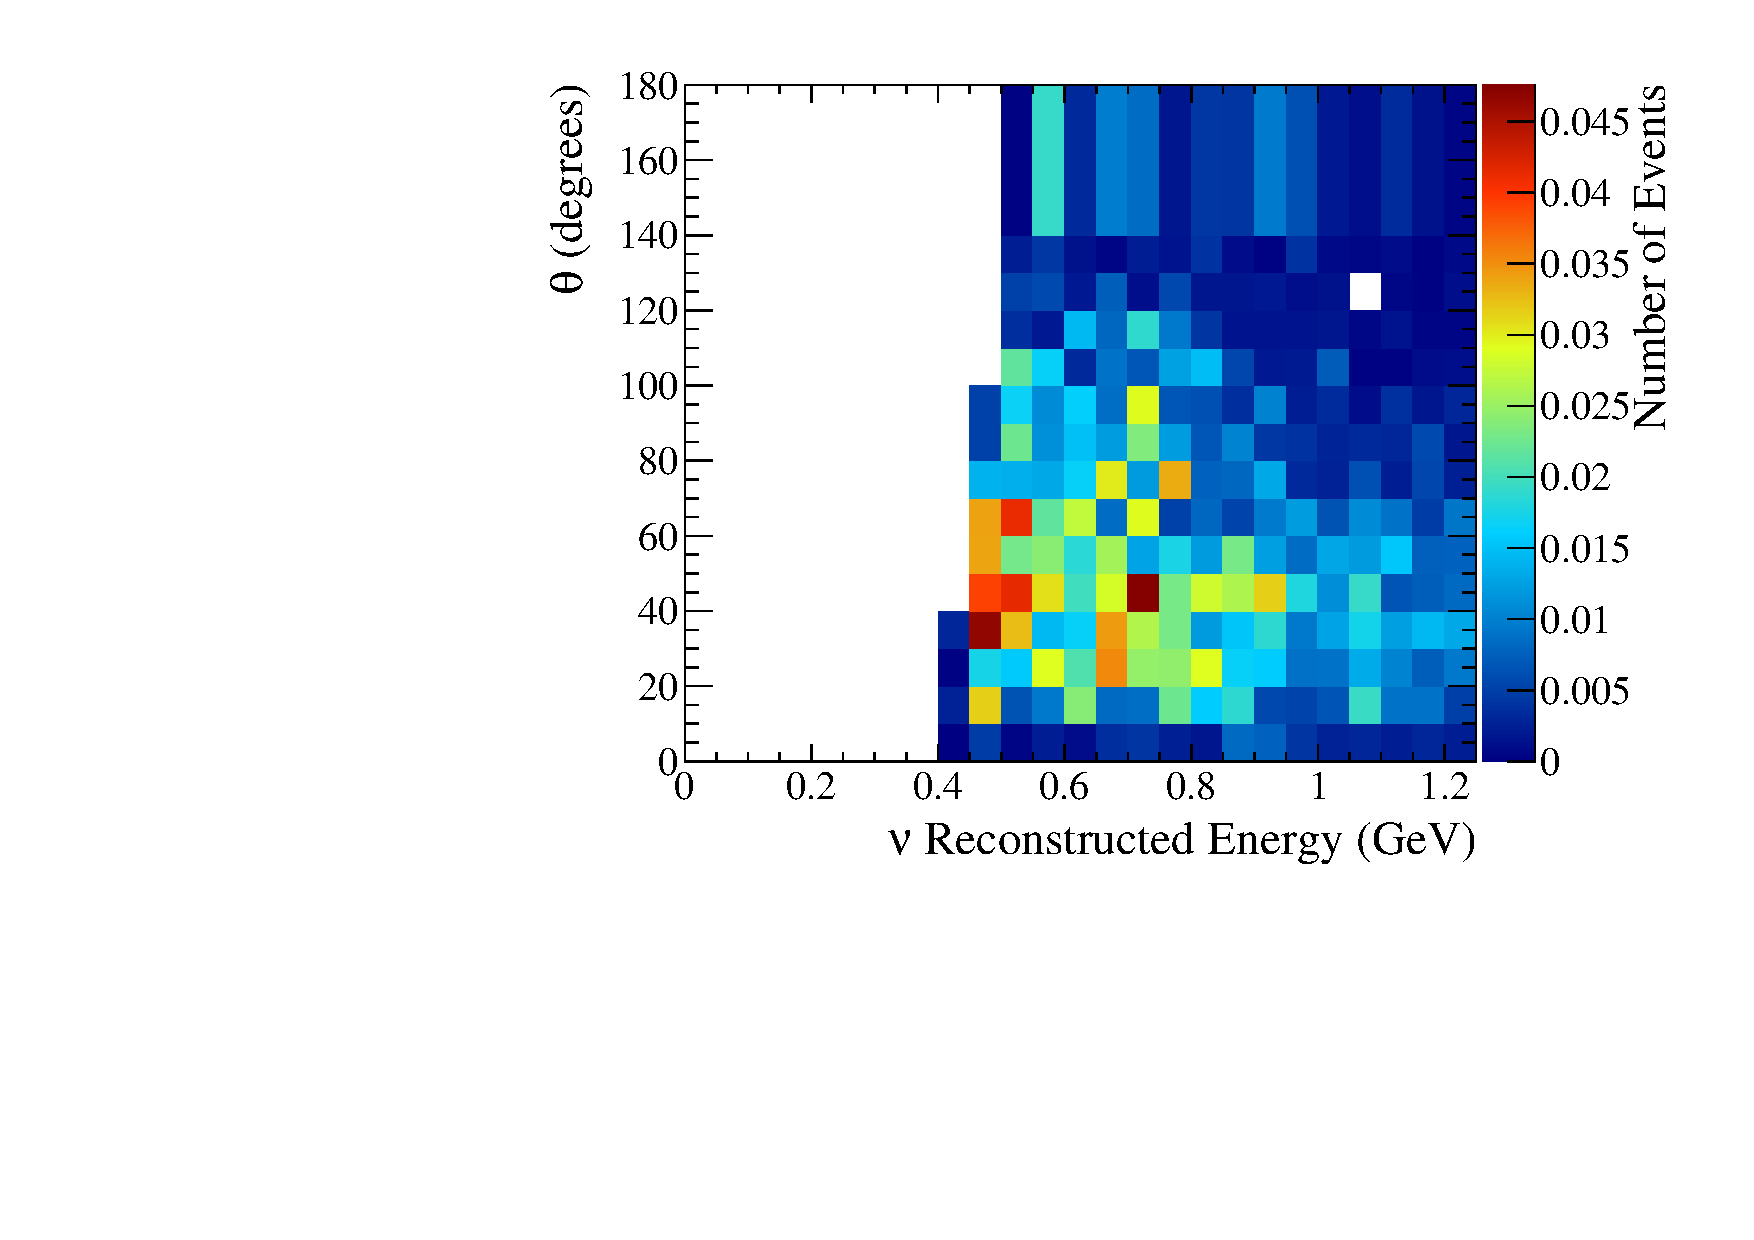
\includegraphics[width=0.9\textwidth]{spectra/spectrum_unosc_MultiRe}
		\caption{\nueCConepi-like, neutrino mode}
	\end{subfigure}
	\caption {
		Predicted unoscillated spectra. $\mu$-like distributions are a function of the reconstructed neutrino energy, while the $e$-like, including \nueCConepi, distributions are functions of both the reconstructed neutrino energy and the reconstructed angle between the outgoing lepton and the neutrino direction. The distributions correspond to the statistics collected in the full \RunPeriod data set. The spectra are generated with the systematic parameters described in \cref{sec:systematics}.
	}
	\label{fig:unosc_spectra_all}
\end{figure*}
\clearpage
\begin{figure*}[htb]
	\center
	\begin{subfigure}[b]{0.49\textwidth}
		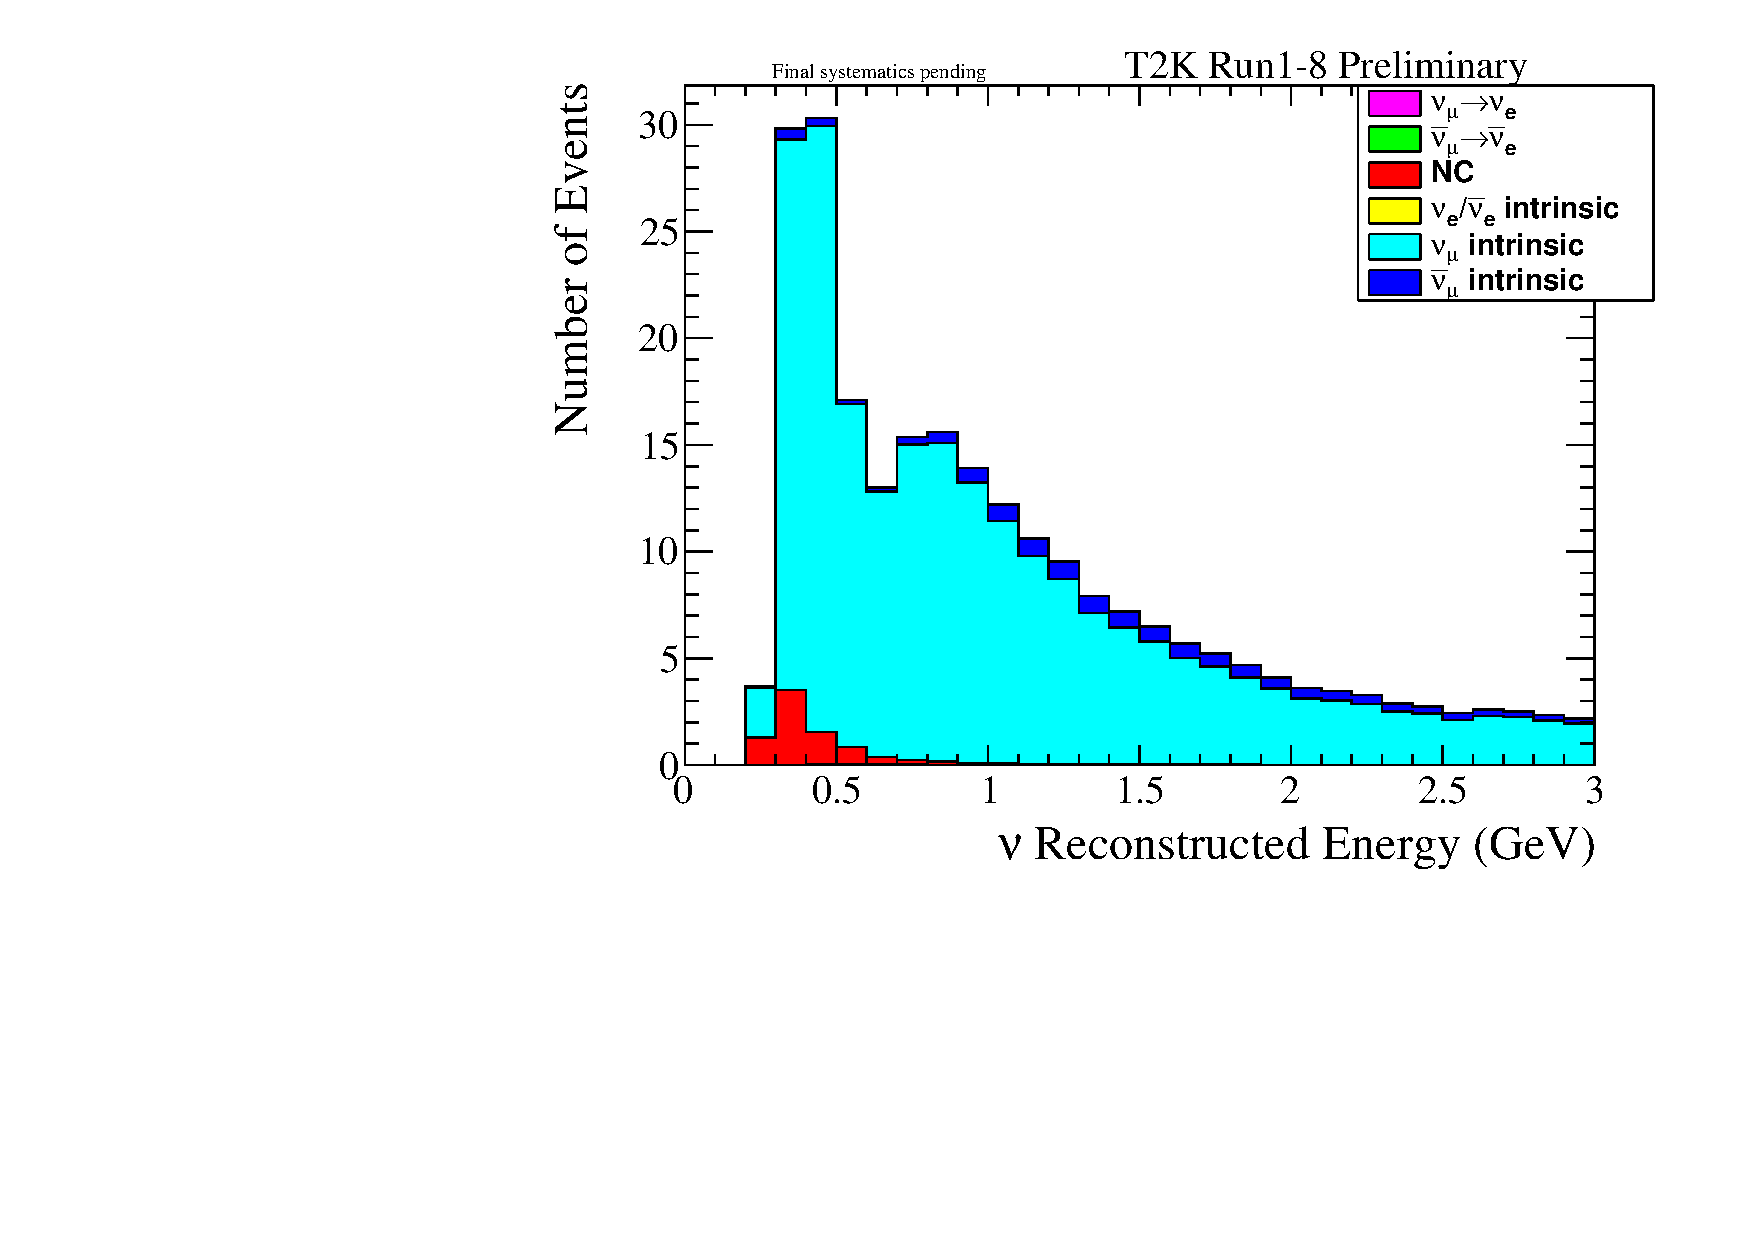
\includegraphics[width=0.9\textwidth]{spectra/spectrum_osc_asimova_1Rmu}
		\caption{Muon-like, neutrino mode}
	\end{subfigure}
	\begin{subfigure}[b]{0.49\textwidth}
		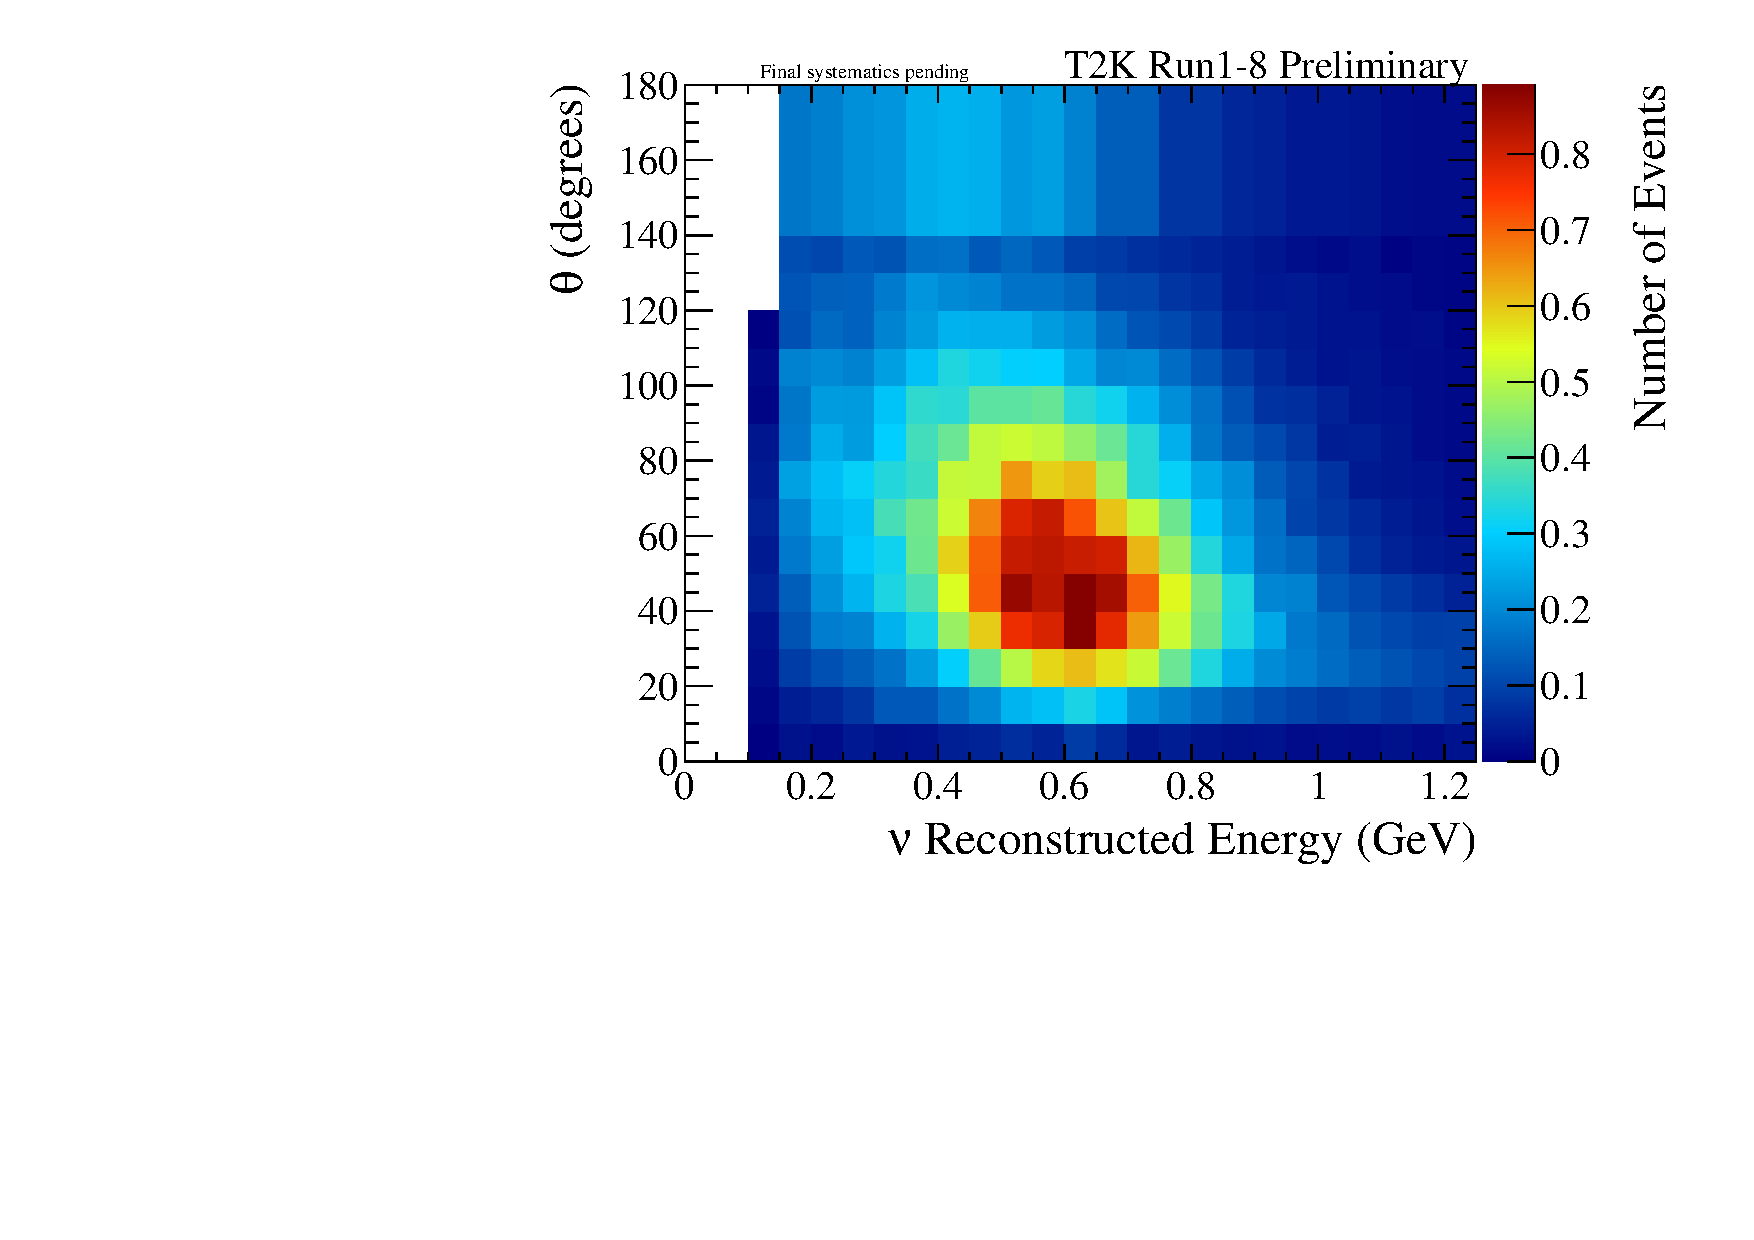
\includegraphics[width=0.9\textwidth]{spectra/spectrum_osc_asimova_1Re}
		\caption{Electron-like, neutrino mode}
	\end{subfigure}
	\begin{subfigure}[b]{0.49\textwidth}
		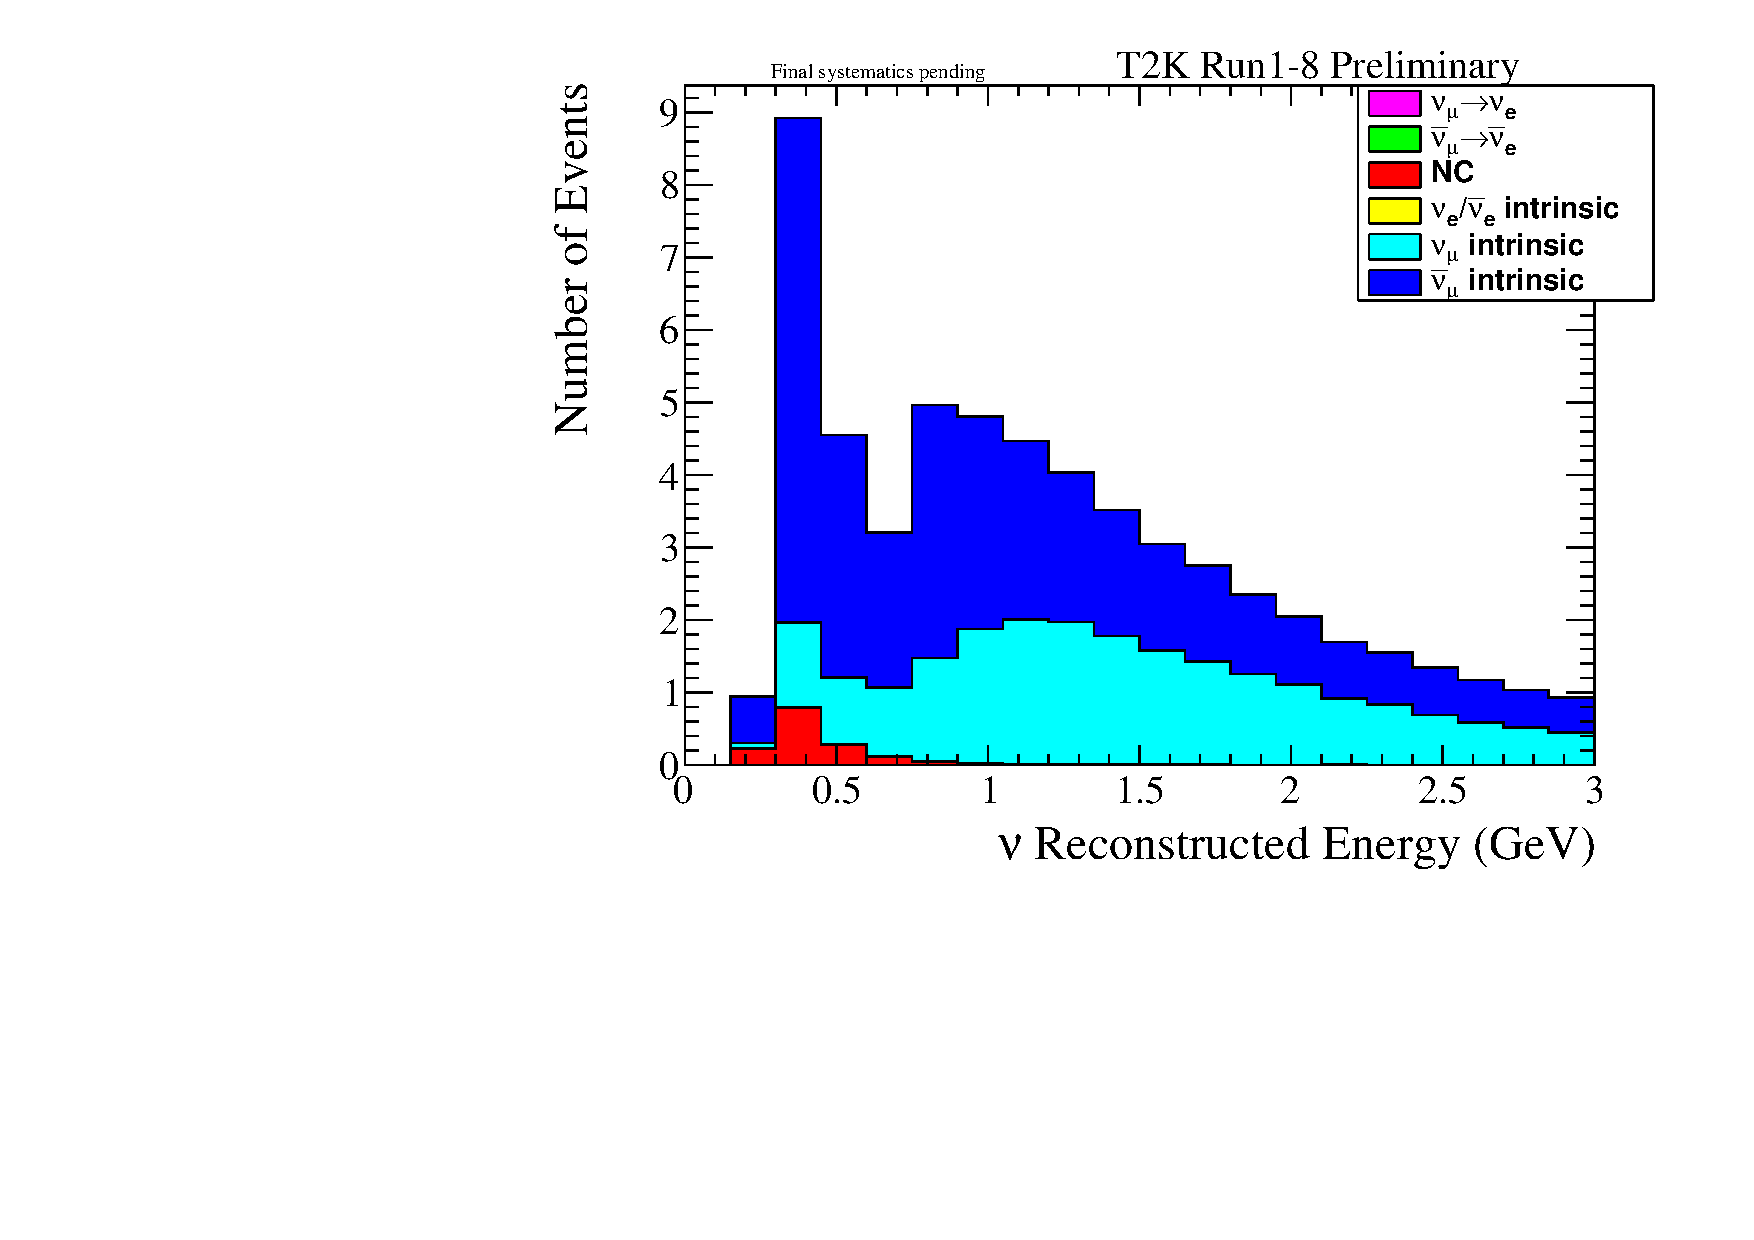
\includegraphics[width=0.9\textwidth]{spectra/spectrum_osc_asimova_RHC1Rmu}
		\caption{Muon-like, antineutrino mode}
	\end{subfigure}
	\begin{subfigure}[b]{0.49\textwidth}
		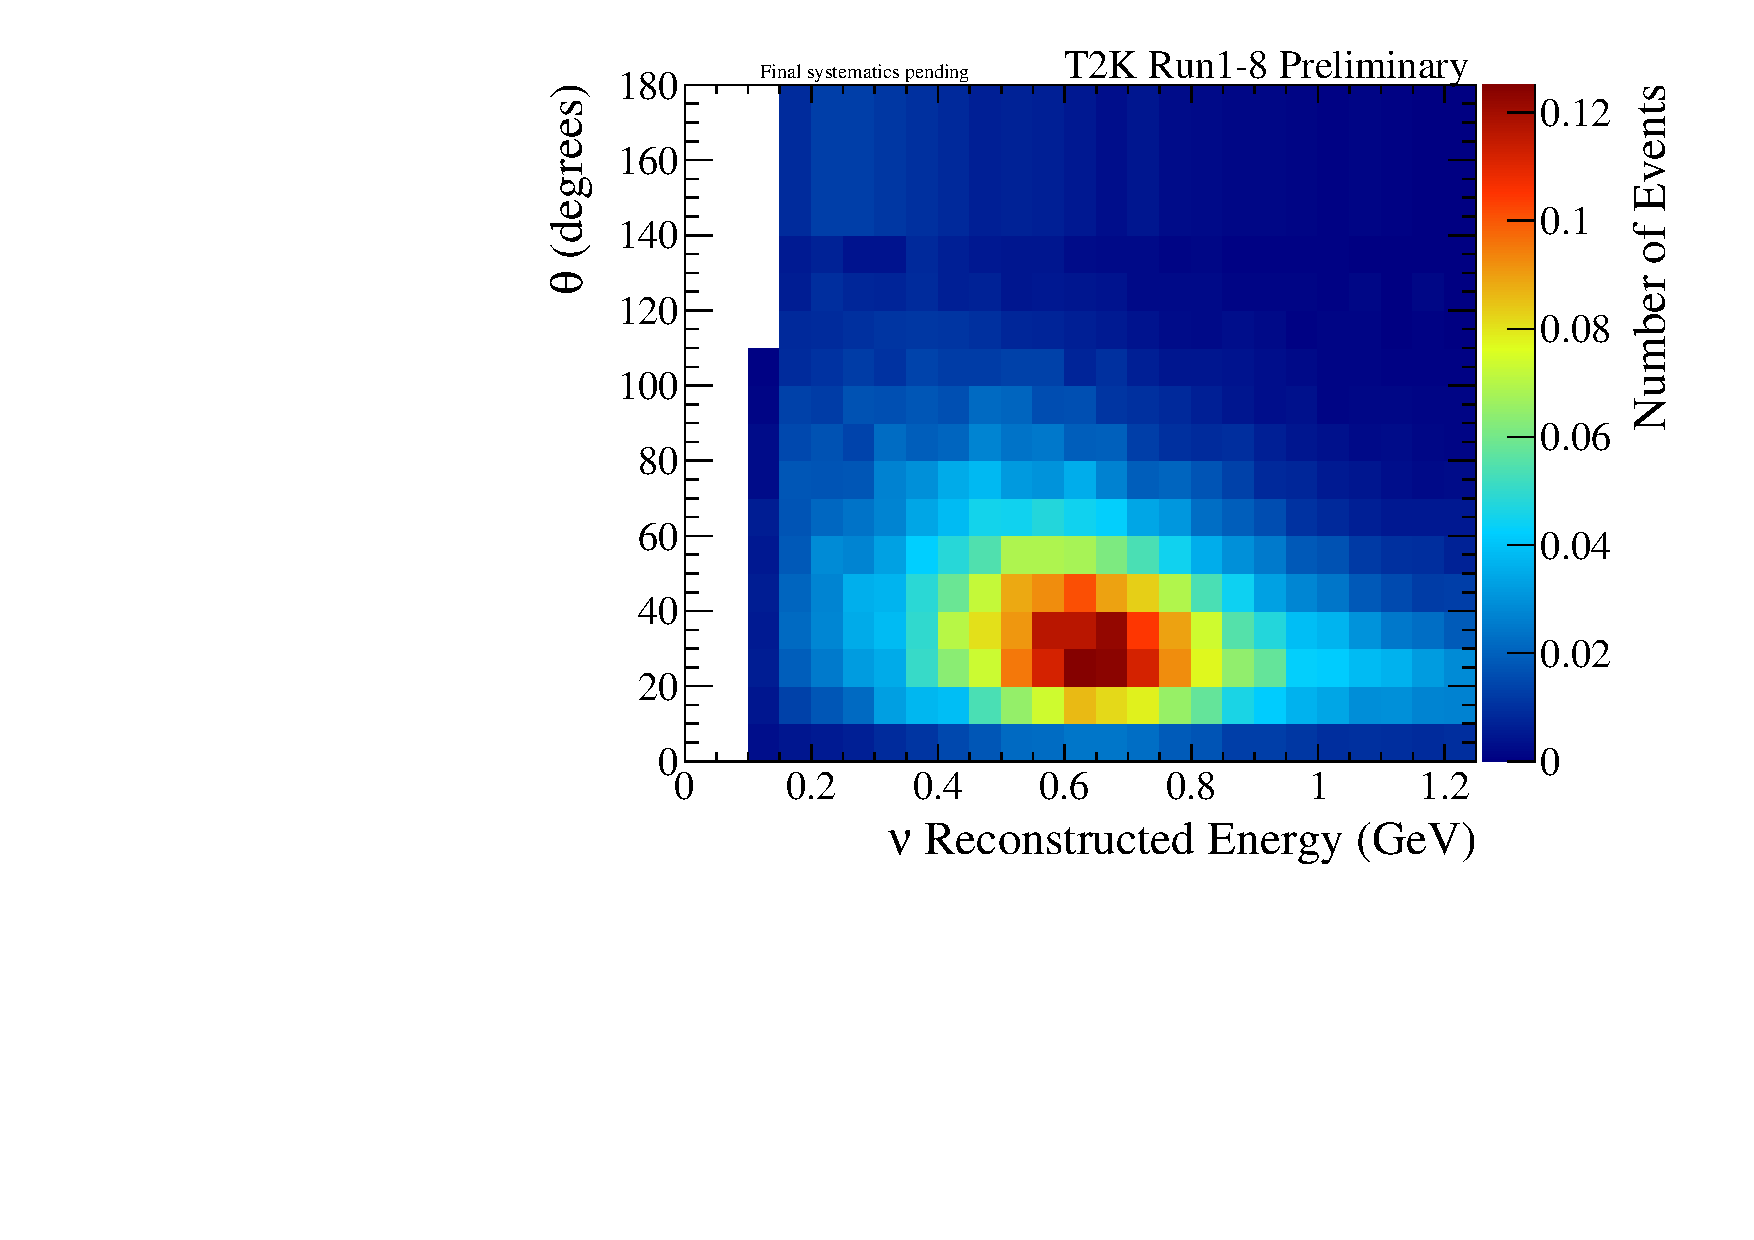
\includegraphics[width=0.9\textwidth]{spectra/spectrum_osc_asimova_RHC1Re}
		\caption{Electron-like antineutrino mode}
	\end{subfigure}
	\begin{subfigure}[b]{0.49\textwidth}
		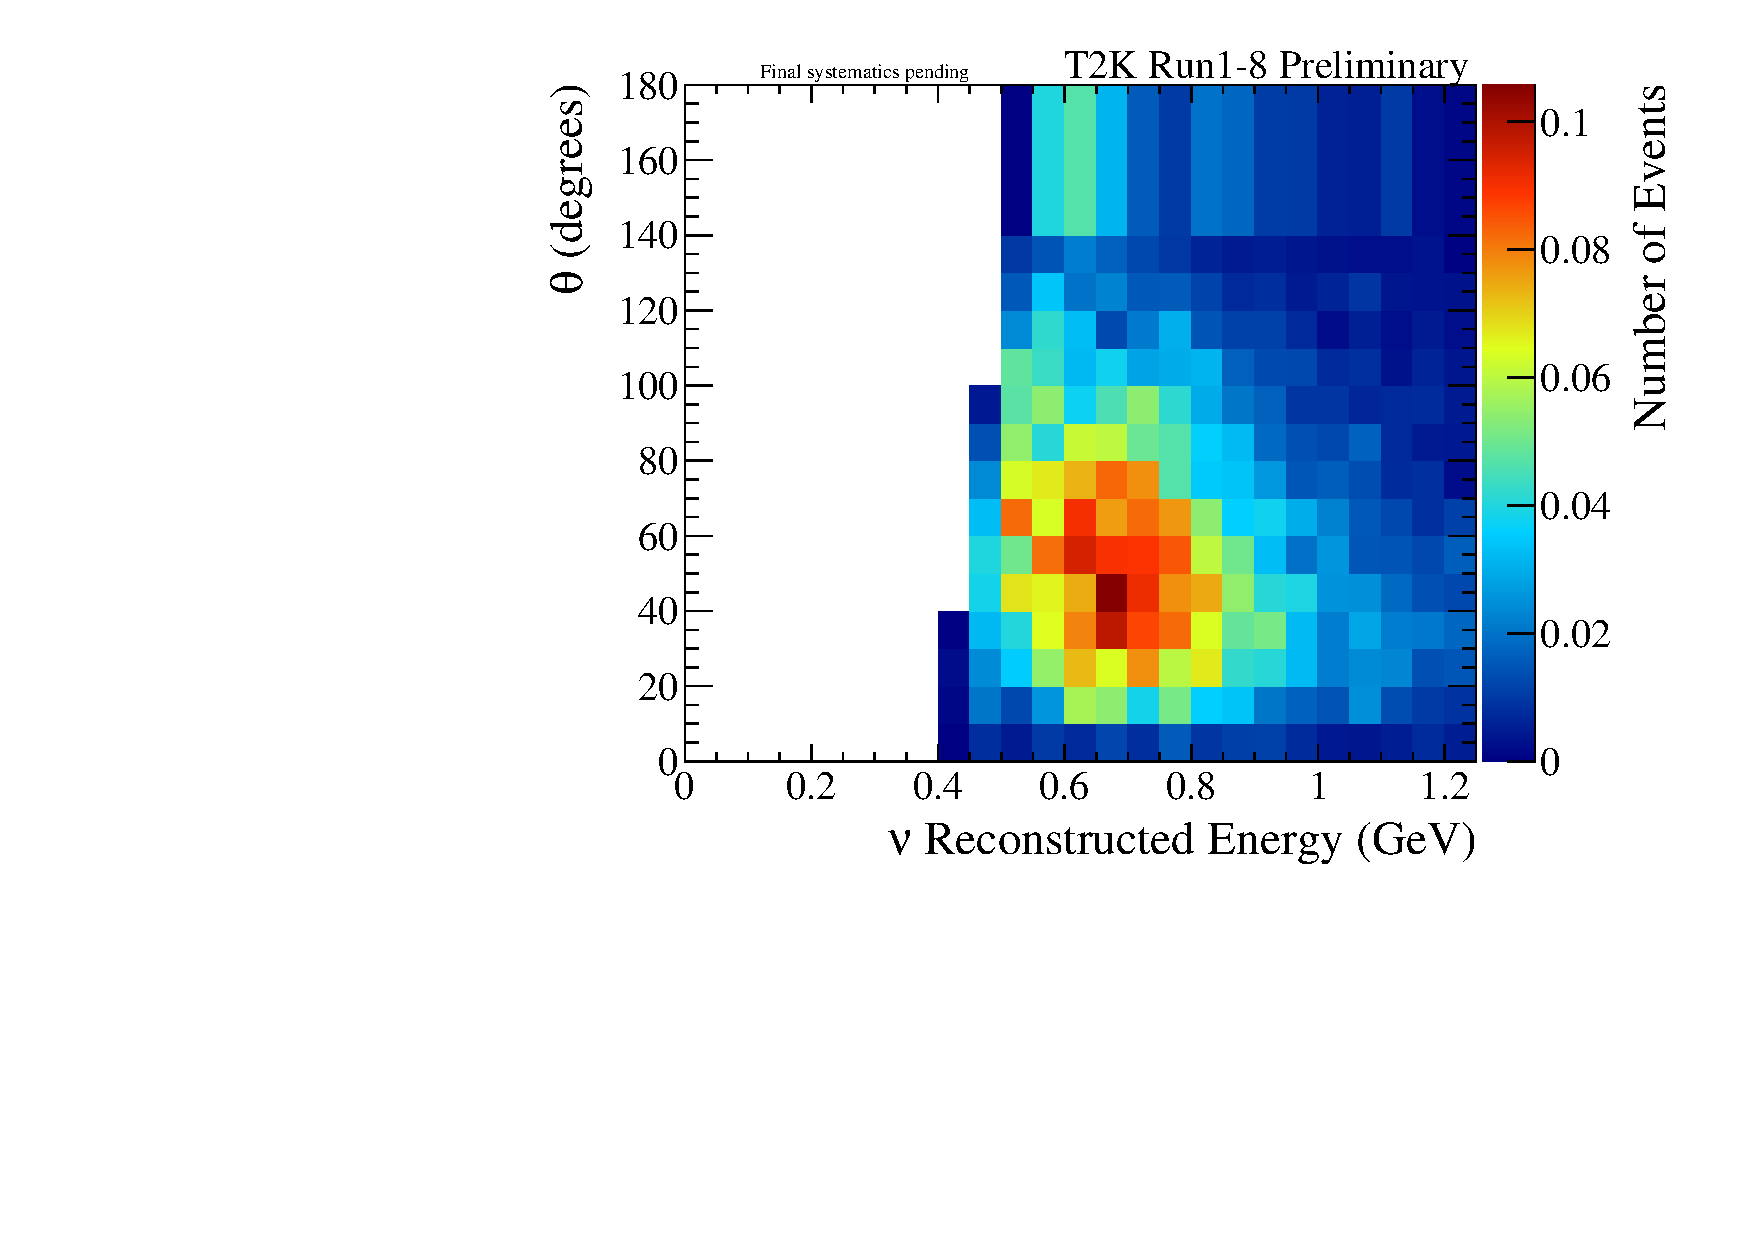
\includegraphics[width=0.9\textwidth]{spectra/spectrum_osc_asimova_MultiRe}
		\caption{\nueCConepi-like, neutrino mode}
	\end{subfigure}
	\caption {
		Predicted Asimov A spectra. $\mu$-like distributions are a function of the reconstructed neutrino energy, while the $e$-like, including \nueCConepi, distributions are functions of both the reconstructed neutrino energy and the reconstructed angle between the outgoing lepton and the neutrino direction. The distributions correspond to the statistics collected in the full \RunPeriod data set. The spectra are generated with the systematic parameters described in \cref{sec:systematics} and the oscillation parameters corresponding to the Asimov data set A shown in \cref{tab:asimov_definition1}.
	}
	\label{fig:asimova_spectra_all}
\end{figure*}
\clearpage

%%% Local Variables:
%%% mode: latex
%%% TeX-master: "../TN327.tex"
%%% End:
